\documentclass[twocolumn,11pt,a4paper]{article}

% Essential packages
\usepackage{lipsum}          % For dummy text
\usepackage{graphicx}        % For including images
\usepackage{amsmath}         % For mathematical equations
\usepackage{amsthm}          % For theorems
\usepackage{booktabs}        % For better tables
\usepackage{microtype}       % For better typography
\usepackage[english]{babel}  % For language settings
\usepackage{geometry}        % For page layout
\usepackage{titlesec}        % For section title formatting
\usepackage{enumitem}        % For customized lists
\usepackage{placeins}        % Add this package

% Chinese font support - add these packages
\usepackage{fontspec}
\usepackage{xeCJK}

% Chinese font configuration
\setmainfont{Sarasa Gothic TC} % Or specify another suitable font like Noto Serif CJK TC
\setCJKmainfont{Sarasa Gothic TC} % Or specify another suitable font like Noto Sans CJK TC
\setCJKsansfont{Sarasa Gothic TC} % Or specify another suitable font like Noto Sans CJK TC
\setCJKmonofont{Sarasa Gothic TC} % Or specify another suitable font like Noto Sans Mono CJK TC

% Page layout
\geometry{
  margin=1.5cm,
  top=1.5cm,
  bottom=2cm,
}

% Set paragraph indentation
\setlength{\parindent}{2em} % Sets indentation to approximately 2 characters width

% Title formatting
\titleformat{\section}
  {\normalfont\large\bfseries}{\thesection}{1em}{}
\titleformat{\subsection}
  {\normalfont\normalsize\bfseries}{\thesubsection}{1em}{}
\titleformat{\subsubsection}
  {\normalfont\normalsize\itshape}{\thesubsubsection}{1em}{} % Added for subsubsection

% Colors for hyperlinks - place after fontspec packages
\usepackage{hyperref}
\hypersetup{
  colorlinks=true,
  linkcolor=blue,
  filecolor=magenta,
  urlcolor=cyan,
  citecolor=green,
}

% Begin document
\begin{document}
% Title page (takes full width)
\twocolumn[
    \begin{@twocolumnfalse}
        \centering
        \vspace{1.5cm}
        {\LARGE\bfseries 軟體工程期中考試書面報告\par}
        \vspace{0.3cm}
        {\small\textit{軟體工程中大語言模型軟體 Kuwa + TAIDE + RAG 和 QCI\&AI 軟硬體整合的應用}\par}
        \vspace{1cm}

        % 作者資訊區塊
        {\large{黃毓峰 - S11159005}\par}
        \vspace{0.3cm}
        {\large 國立臺南大學 資訊工程學系\par}
        \vspace{0.3cm}
        {\large a288235403@gmail.com\par}
        \vspace{0.3cm}
        {\large 指導教授:李健興 教授\par}
        \vspace{0.5cm}

        {\large \today\par}
        \vspace{1cm}
    \end{@twocolumnfalse}
]

% Abstract
\section*{摘要}
本報告旨在整合軟體工程 (Software Engineering) 的核心概念與
量子計算智慧暨人工智慧 (Quantum Computational Intelligence \& Artificial Intelligence, QCI\&AI) 學習工具的實作經驗,
以建立一個兼具理論與實務的綜合學習框架。透過回顧 Sommerville 的《Software Engineering》教科書前四章的關鍵知識點,
並詳述 Kuwa 平台、大型語言模型 (LLM) API 與本地模型部署的過程,以及檢索增強生成 (Retrieval-Augmented Generation, RAG) 功能的應用,
本報告展示了如何將軟體工程原則應用於 QCI\&AI 領域的學習與探索,
特別是在數據收集、推論模型建立與微調模型的學習階段中。本報告也強調了軟體工程在 QCI\&AI 學習中的重要性,並將軟體工程的原則應用於數據收集、推論模型建立和微調模型的學習階段。
\linebreak \linebreak 
\noindent \textbf{關鍵字:} 軟體工程、量子計算智慧、人工智慧、大型語言模型、檢索增強生成

\section*{Abstract}
This report aims to integrate the core concepts of Software Engineering with the practical experience of 
implementing Quantum Computational Intelligence \& Artificial Intelligence (QCI\&AI) learning tools, 
establishing a comprehensive learning framework that combines theory and practice. 
By reviewing the key knowledge points from the first four chapters of Sommerville's "Software Engineering" 
textbook, detailing the process of deploying the Kuwa platform, Large Language Model (LLM) APIs,
and local models, and applying Retrieval-Augmented Generation (RAG) functionality, 
this report demonstrates how to apply software engineering principles to learning and exploring the QCI\&AI field, 
particularly in the learning stages of data collection, inference model building, and fine-tuning models. 
The report also emphasizes the importance of software engineering in QCI\&AI learning and 
applies software engineering principles to the learning stages of data collection, 
inference model building, and fine-tuning models.
\linebreak \linebreak
\noindent \textbf{Keywords:} Software Engineering, Quantum Computational Intelligence, Artificial Intelligence, Large Language Models, Retrieval-Augmented Generation


% Introduction
\section{Introduction}
隨著資訊科技的飛速發展,軟體系統已滲透到現代社會的各個角落,從日常生活的應用程式到關鍵基礎設施的控制系統,
軟體工程 (Software Engineering) 的重要性不言而喻。建立可靠、高效且易於維護的軟體系統,
是所有已開發國家經濟發展的基石。與此同時,人工智慧 (Artificial Intelligence, AI) 與量子計算 (Quantum Computing) 的融合,
催生了量子計算智慧 (Quantum Computational Intelligence, QCI) 這個新興領域,為解決複雜問題帶來了全新的可能性。
然而,對於初學者或學生而言,如何在掌握傳統軟體工程基礎知識的同時,有效地學習和應用這些前沿的 QCI\&AI 技術,往往是一大挑戰。

理論知識與實際操作之間存在的鴻溝,可能阻礙學習者深入探索這些領域。
本報告旨在搭建一座橋樑,連接軟體工程的基礎理論與 QCI\&AI 技術的實務應用。
報告的主要目的有二:第一,系統性地回顧軟體工程的核心概念,內容依據 Sommerville 的《Software Engineering》教科書前四章 \cite{sommerville2015},
涵蓋軟體工程導論、軟體流程、敏捷開發及需求工程等關鍵主題。第
二,詳細介紹一套 QCI\&AI 軟硬體學習工具的具體實作流程,包括 Kuwa 平台的安裝設定(涵蓋 Windows 與 Linux/Docker 環境)、雲端 Gemini Pro API 的整合、
本地端 GGUF 模型的部署方法,以及 RAG 功能的初步應用。並結合 IEEE SSCI 2025 工作坊所倡導的學習階段(數據收集、推論模型、微調模型),展示如何將理論應用於實踐。
透過此整合框架,期望能為學習者提供一條更清晰的路徑,以應對未來軟體開發與 AI 技術融合的挑戰。

% Section: Software Engineering Core Concepts
\section{軟體工程核心概念回顧}
本節回顧 Sommerville \cite{sommerville2015} 教科書前四章的核心概念,為後續討論 QCI\&AI 工具的應用奠定理論基礎。

\subsection{軟體工程導論 (Chapter 1)}
軟體工程是一門關注所有軟體生產相關方面的工程學科。它不僅僅是技術性的程式設計,更涵蓋了從早期系統規格定義到系統部署後維護的完整過程。
好的軟體應具備以下關鍵屬性:
\begin{itemize}[noitemsep, topsep=0pt,leftmargin=*]
    \item \textbf{可維護性 (Maintainability)}:軟體需能演進以滿足客戶變化的需求。
    \item \textbf{可靠性與安全性 (Dependability and Security)}:軟體應穩定運行,不應在失敗時造成物理或經濟損害,並能抵禦惡意訪問。
    \item \textbf{效率 (Efficiency)}:軟體不應浪費系統資源,如記憶體和處理器週期。
    \item \textbf{可接受性 (Acceptability)}:軟體必須對其目標用戶群體是可理解、可用且兼容的。
\end{itemize}
軟體工程需要應對異質性 (Heterogeneity)、業務和社會變革 (Business and social change) 以及安全和信任 (Security and trust) 等挑戰。

\subsection{軟體流程 (Chapter 2)}
軟體流程 (Software Process) 是指創建高品質軟體所需的一系列結構化活動集合。常見的軟體流程模型包括:
\begin{itemize}[noitemsep, topsep=0pt]
    \item \textbf{瀑布模型 (Waterfall Model)}:計劃驅動,具有明確定義的階段(需求分析、設計、實現、測試、維護)。其主要缺點是難以適應變更。
    \item \textbf{增量開發 (Incremental Development)}:規格定義、開發和驗證交錯進行。能更快交付可用軟體,更容易獲得客戶反饋,但過程可能不夠透明。
    \item \textbf{整合與配置 (Integration and Configuration)}:基於現有可配置元件組裝系統,強調軟體重用 (Software Reuse)。
\end{itemize}
現實中的大型專案往往混合使用這些模型的元素。流程活動包括軟體規格定義 (Software Specification)、軟體設計與實現 (Software Design and Implementation)、軟體驗證 (Software Validation) 和軟體演進 (Software Evolution)。應對變更是軟體工程中的核心挑戰,而流程改進 (Process Improvement) 對於提升軟體品質至關重要。

\subsection{敏捷開發 (Chapter 3)}
敏捷方法 (Agile Methods) 是為了應對快速變化的需求而生,強調快速交付、客戶協作和對變化的響應。其核心價值觀體現在《敏捷宣言》中:
\begin{itemize}[noitemsep, topsep=0pt]
    \item 個體與互動 \textbf{重於} 流程與工具。
    \item 可工作的軟體 \textbf{重於} 詳盡的文件。
    \item 客戶合作 \textbf{重於} 合約協商。
    \item 回應變化 \textbf{重於} 遵循計劃。
\end{itemize}
敏捷原則包括客戶滿足、擁抱變化、頻繁交付、業務人員與開發者合作、建立積極的環境、面對面溝通、可工作的軟體是主要進度量度、可持續的開發步調、持續關注技術卓越和良好設計、簡潔性、自組織團隊以及定期反思調整。
極限編程 (Extreme Programming, XP) 是一種有影響力的敏捷方法,其核心實踐包括增量規劃 (Incremental Planning)、小型發布 (Small Releases)、簡單設計 (Simple Design)、測試驅動開發 (Test-first Development)、重構 (Refactoring)、配對編程 (Pair Programming)、集體所有權 (Collective Ownership)、持續整合 (Continuous Integration)、可持續步調 (Sustainable Pace) 和現場客戶 (On-site Customer)。
敏捷方法適用於需求易變的中小型產品開發,但在大型系統或需要大量前期分析的系統中應用面臨挑戰。

\subsection{需求工程 (Chapter 4)}
需求工程 (Requirements Engineering) 是發現、分析、記錄和檢查系統所需服務和約束的過程。需求分為:
\begin{itemize}[noitemsep, topsep=0pt]
    \item \textbf{用戶需求 (User Requirements)}:以自然語言和圖表描述,供客戶閱讀。
    \item \textbf{系統需求 (System Requirements)}:更詳細地描述系統功能、服務和操作约束,是系統合約的一部分。
\end{itemize}
功能需求 (Functional Requirements) 描述系統應提供的服務或功能。非功能需求 (Non-functional Requirements) 是對系統或開發過程的約束,如性能、安全性或可靠性。
需求工程過程是一個迭代的螺旋模型,包括:
\begin{enumerate}[noitemsep, topsep=0pt]
    \item \textbf{需求獲取 (Requirements Elicitation/Discovery)}:與利益相關者 (Stakeholders) 互動以了解需求。常用技術包括訪談 (Interviews)、場景 (Scenarios)、用戶故事 (User Stories) 和民族誌 (Ethnography)。
    \item \textbf{需求分類與組織 (Requirements Classification and Organization)}:將混亂的需求結構化。
    \item \textbf{需求優先級排序與協商 (Requirements Prioritization and Negotiation)}:解決需求衝突。
    \item \textbf{需求規格說明 (Requirements Specification)}:將需求記錄在《軟體需求規格說明書》(Software Requirements Specification, SRS) 中。SRS 應力求完整 (Complete) 和一致 (Consistent)。
    \item \textbf{需求驗證 (Requirements Validation)}:檢查需求的有效性、一致性、完整性、現實性和可驗證性。常用技術包括需求審查 (Requirements Reviews) 和原型開發 (Prototyping)。
    \item \textbf{需求管理 (Requirements Management)}:在開發過程中管理變更的需求。
\end{enumerate}

\section{QCI\&AI 學習工具實作}

\subsection{軟硬體環境設定}

本節說明如何進行 Thonny 軟體安裝與設定,並將 QCI\&AI 學習工具連接至個人電腦,透過 Python 程式進行資料蒐集。

\begin{itemize}
    \item 下載並安裝 Thonny 4.1.7 軟體環境。
    \item 設定 Thonny 使用 MicroPython (generic) 模式,並選取正確的通訊埠 (COM Port)。
    \item 將 QCI\&AI 學習工具透過 USB 接上個人電腦,並啟動工具。
    \item 使用 Thonny 執行 QCIGAIModel\_DataCollection.py 進行資料收集,擷取影像及距離、光線資訊。
\end{itemize}

\subsection{模糊集合與模糊系統實作}

利用 QCI\&AI 學習工具與 KWS AI 平台進行資料蒐集與處理:

\begin{itemize}
    \item 使用學習工具拍攝並儲存影像及相應的距離 (Distance)、光線 (Light) 數據。
    \item 上傳影像至 KWS AI 平台生成中英文文字描述 (GAIText) 及對應的影像 (GAIImage)。
    \item 進行人類主觀評估,計算 HEGAIText、HEGAIImage 分數,進一步生成 GAIFit 值。
    \item 定義模糊變數與語意項 (Linguistic Terms),建立模糊變數距離 (near, medium, far)、光線 (dark, medium, bright)、HEGAIText 與 HEGAIImage (low, medium, high) 和 GAIFit (poor, medium, good) 的語意項函數。
\end{itemize}

\subsection{模糊推理模型建構與驗證}

依據前面定義的模糊語意項建構模糊推理模型:

\begin{itemize}
    \item 建立推理規則集,載入至 QCI\&AI-FML 學習平台。
    \item 利用推理模型進行資料推論與驗證,包含手動及批次資料推論。
    \item 使用 MQTT 連接,將推論結果傳送至學習工具進行硬體反應測試。
    \item 專家模型驗證,包括計算語意匹配準確度、均方誤差 (MSE)、均方根誤差 (RMSE)。
\end{itemize}

\subsection{演化計算與模型微調}

透過演化計算 (PSO 粒子群最佳化) 進行知識模型的微調與最佳化:

\begin{itemize}
    \item 載入訓練數據,設定粒子數與迭代次數,進行模型訓練。
    \item 透過訓練過程中的準確率、MSE 曲線觀察模型的優化效果。
    \item 比較訓練前後知識模型,保存並驗證最佳化後的模型。
\end{itemize}

\subsection{量子模糊推理引擎實作}

使用量子計算智能 (Quantum Computational Intelligence, QCI) 方法進行模糊推理:

\begin{itemize}
    \item 將傳統模糊推理模型轉換為基於量子電路的量子推理模型。
    \item 使用 IBM Quantum Simulator 進行量子推理模型的模擬與執行。
    \item 分析量子推理結果,包含量子電路實現、計數圖 (Count Chart)、機率圖 (Probability Chart) 及量子推理與傳統推理結果的比較。
    \item 驗證量子推理方法於 QCI\&AI 學習工具上的實際硬體應用。
\end{itemize}


\section{KUWA+TAIDE+RAG 安裝實作內容}
本節介紹一套用於學習 QCI\&AI 的軟硬體工具的安裝與設定流程,主要基於 Kuwa 平台,並整合雲端與本地大型語言模型。

\subsection{Kuwa 平台安裝與設定}
Kuwa GenAI OS 是一個提供與大型語言模型 (LLM) 互動環境的平台。其安裝方式因操作系統而異。

\textbf{Windows 環境:} 根據提供的 Windows 版本安裝指引 (v.0.9) 和 KUWA TAIDE v0.2.0 安裝手冊,主要步驟包括:
\begin{enumerate}[noitemsep, topsep=0pt]
    \item \textbf{環境準備}:安裝 Microsoft Visual C++ 可轉散發套件,以及(若使用 GPU)對應版本的 NVIDIA CUDA Toolkit。
    \item \textbf{下載 Kuwa}:從指定網址下載對應 CPU 或 GPU (CUDA 版本) 的 `.exe` 執行檔,或從 GitHub 獲取源碼。
    \item \textbf{執行與啟動}:執行 `.exe` 文件或相關啟動腳本 (`build.bat`, `start.bat`)。系統會啟動本地伺服器,通常可通過瀏覽器訪問 `http://localhost:8080`。
\end{enumerate}

\textbf{Linux 環境 (基於 Docker):} 另一種常見方式是在 Linux 環境(如 Ubuntu VM)中使用 Docker 進行部署。此方法更靈活但也更複雜,尤其在需要利用主機 GPU 資源時:
\begin{enumerate}[noitemsep, topsep=0pt]
    \item \textbf{環境準備}:建立虛擬機 (如使用 QEMU/KVM),配置 GPU Passthrough(涉及 IOMMU 啟用、`vfio-pci` 模組加載、啟動/停止掛鉤腳本設定等複雜步驟),並在 VM 內安裝 Docker、NVIDIA 驅動及 NVIDIA Container Toolkit。
    \item \textbf{下載與配置 Kuwa}:克隆 `genai-os` GitHub 倉庫。
    \item \textbf{構建與運行容器}:根據需求拉取或構建 Docker 鏡像(例如,為 GPU 使用拉取 `kuwaai/model-executor:v0.3.4-cu121` 並標記為 `latest`),並使用 Docker Compose(通過修改 `run.sh` 執行多個 `.yaml` 配置文件)來啟動 Kuwa 的各個服務容器。
\end{enumerate}
不論何種安裝方式,Kuwa 平台都提供了一個儀表板 (Dashboard),包含聊天 (Chat) 和房間 (Room) 等功能。Room 功能允許用戶創建一個包含多個 LLM 的對話空間,方便進行模型比較。

\subsection{雲端 LLM API 整合 (Gemini Pro)}
Kuwa 平台支援串接外部的 LLM API,例如 Google Gemini Pro。整合步驟如下:
\begin{enumerate}[noitemsep, topsep=0pt]
    \item \textbf{獲取 API 金鑰}:前往 Google AI Studio (\url{ai.google.dev}) 申請並獲取 Gemini API 金鑰。
    \item \textbf{配置 Kuwa}:在 Kuwa 平台的界面中,通常在個人設定 (Profile) 或相關設定頁面,找到 API 金鑰輸入欄位,將獲取的 Gemini API 金鑰填入。
    \item \textbf{測試連接}:保存設定後,在聊天界面選擇 Gemini Pro 模型,發送訊息進行測試,確認是否能成功接收回覆。
\end{enumerate}
同樣的流程也適用於整合 OpenAI ChatGPT 等其他雲端 API。

\subsection{本地 GGUF 模型部署 (Llama.cpp)}
Kuwa 也支援透過 Llama.cpp 等後端運行本地的大型語言模型,常見格式為 GGUF (GPT-Generated Unified Format)。部署方式根據 Kuwa 的安裝環境有所不同:

\textbf{Windows 環境 (基於 \texttt{env.bat}):}
\begin{enumerate}[noitemsep, topsep=0pt]
    \item \textbf{下載 GGUF 模型}:從 Hugging Face 等模型庫下載所需的 GGUF 格式模型檔案。
    \item \textbf{配置環境變數}:編輯 Kuwa 目錄下的 \texttt{env.bat} 文件。找到 \texttt{gguf\_path} 相關的行,取消註解並填寫下載的 GGUF 模型檔案的完整路徑。
    \item \textbf{重新啟動 Kuwa}:關閉並重新執行 `start.bat`。
    \item \textbf{選擇模型}:在 Kuwa 儀表板的模型選擇列表中,應會出現 LLaMA.cpp Model 或類似選項。
\end{enumerate}

\textbf{Linux 環境 (基於 Docker Compose):}
\begin{enumerate}[noitemsep, topsep=0pt]
    \item \textbf{下載 GGUF 模型}:同上。
    \item \textbf{創建 Docker Compose 配置}:在 \texttt{compose} 目錄下為目標模型創建一個新的 \texttt{.yaml} 文件
    (例如 \texttt{llama-3.1-taide-lx-8b-chat.yaml})。在此文件中定義服務,指定使用 \texttt{kuwaai/model-executor} 鏡像,
    設置環境變數(如 \texttt{EXECUTOR\_TYPE: llamacpp}, 模型名稱、圖片等),並通過 volumes 將本地模型文件映射到容器內的 \texttt{/var/model/}
     路徑。如果使用 GPU,需在 \texttt{deploy.resources.reservations.devices} 中指定 GPU 資源。
    \begin{enumerate}[noitemsep, topsep=0pt]
        \item \textbf{修改啟動腳本}:編輯 `run.sh` 文件,在 `confs` 數組中加入新創建的 Compose 文件名(不含 `.yaml` 後綴)。
    \end{enumerate}
    \item \textbf{重新啟動 Kuwa}:執行 `./run.sh`。
    \item \textbf{選擇模型}:在 Kuwa 儀表板中選擇新配置的模型。
\end{enumerate}
使用本地模型可以在沒有網路連接或需要更高隱私性的情況下運行 LLM。但需要注意本地模型的性能(尤其是中文處理能力)可能不如大型雲端模型,且對硬體資源有一定要求。

\subsection{RAG 功能應用} % New subsection based on Homework 4
檢索增強生成 (Retrieval-Augmented Generation, RAG) 是 Kuwa 的一項重要功能,允許 LLM 結合外部知識庫進行回答。在 Windows 環境下設定 RAG 的基本步驟如下:
\begin{enumerate}[noitemsep, topsep=0pt]
    \item \textbf{環境準備}:
        \begin{itemize}[noitemsep, topsep=0pt]
            \item (可能需要) 運行 Kuwa 目錄下的 \texttt{tool.bat} 進行模式切換(例如切換到 CPU 模式)。
            \item 安裝特定版本的 Python 依賴:`pip uninstall numpy faiss-cpu` 後執行 `pip install numpy==1.24.4 faiss-cpu==1.7.4`。
        \end{itemize}
    \item \textbf{構建知識庫}:準備包含知識文件的資料夾(例如,包含 xLSTM 相關文件的資料夾),並將該資料夾拖曳到 Kuwa 提供的「Construct RAG」捷徑上,以建立向量索引。
    \item \textbf{配置 RAG Bot}:
        \begin{itemize}[noitemsep, topsep=0pt]
            \item 進入 Kuwa 儀表板的「Store」(商店) 頁面。
            \item 選擇剛剛建立的 RAG Bot (如果未出現可能需要重啟 Kuwa)。
            \item 在「Model config file」中指定用於生成答案的 LLM,例如輸入 \texttt{PARAMETER generator\_model ``llama-3-1-taide''}。
            \item 保存設定。
        \end{itemize}
    \item \textbf{開始問答}:完成配置後,即可在聊天界面與該 RAG Bot 進行互動,它會根據您提供的知識庫內容來回答問題。
\end{enumerate}
此 RAG 功能使得 LLM 能夠利用特定領域的最新資訊,提高了回答的準確性和相關性。

% Section: Bridging Theory and Practice
\section{理論與實務的結合:SE 於 QCI\&AI 學習}
將軟體工程的理論應用於 QCI\&AI 工具的學習與實踐,可以使學習過程更結構化、更有效率。以下結合 IEEE SSCI 2025 工作坊倡導的學習階段進行探討。

\subsection{數據收集階段 (Data Collection)}
此階段對應軟體工程中的\textbf{需求工程}。在使用 Kuwa 和 LLM 進行特定任務(例如建立一個問答機器人或使用 RAG)時:
\begin{itemize}[noitemsep, topsep=0pt]
    \item \textbf{需求獲取}:明確學習目標或任務需求。需要收集哪些類型的數據(用於 RAG 的文檔,或用於評估模型的問答對)?模型的預期輸入和輸出是什麼?這類似於定義用戶需求和系統需求。
    \item \textbf{數據規格說明}:定義數據的格式、來源和質量要求(例如 RAG 文檔的結構),類似於編寫需求規格說明書。
    \item \textbf{利益相關者分析}:如果是在團隊中學習,需要識別不同成員的目標和期望。
\end{itemize}
使用 Kuwa 的聊天功能與不同模型互動,或準備 RAG 的知識庫,本身就是一種數據收集和需求探索的過程。

\subsection{推論模型階段 (Inference Model)}
此階段涉及使用預訓練模型進行推理(包括 RAG),對應軟體工程中的\textbf{軟體設計與實現}和\textbf{軟體驗證}。
\begin{itemize}[noitemsep, topsep=0pt]
    \item \textbf{模型/架構選擇 (設計)}:根據任務需求(功能需求)和資源限制(非功能需求,如響應時間、成本、隱私、是否需要特定知識),選擇使用雲端 API (Gemini)、本地模型 (TAIDE GGUF),或配置 RAG。這類似於軟體架構設計中的技術選型。
    \item \textbf{整合與配置 (實現)}:按照前述步驟安裝 Kuwa、配置 API 金鑰、本地模型路徑或 RAG 知識庫。這是一個典型的系統整合過程。
    \item \textbf{測試與驗證}:透過 Kuwa 的聊天或房間功能,向選定的模型或 RAG Bot 發送測試輸入,評估其輸出是否符合預期(功能驗證)。比較不同模型或 RAG 配置的回覆質量、速度和風格(非功能驗證)。這類似於單元測試和系統測試。
    \item \textbf{敏捷迭代}:如果模型效果不佳,可以快速切換到另一個模型,調整輸入提示 (Prompt Engineering),或更新 RAG 知識庫並重建索引,體現了敏捷開發中快速響應變化的思想。
\end{itemize}

\subsection{微調模型階段 (Fine-tuning Model)}
雖然本報告涉及的工具主要側重於使用預訓練模型和 RAG,但微調的概念對應軟體工程中的\textbf{軟體演進}和\textbf{維護}。
\begin{itemize}[noitemsep, topsep=0pt]
    \item \textbf{需求變更管理}:當發現預訓練模型或 RAG 在特定領域或任務上表現不足時,就產生了「微調」的需求,這類似於軟體演進中因需求變更而進行的修改。
    \item \textbf{增量開發}:微調通常是一個迭代過程,收集特定數據、訓練、評估,再根據結果調整,符合增量開發的理念。
    \item \textbf{可維護性}:選擇易於微調的模型架構和工具鏈,關係到未來模型維護的難易度。
\end{itemize}
即使不進行實際的微調,理解其過程也有助於認識到模型像軟體一樣,需要持續的維護和改進以適應新的需求和數據。

\subsection{軟體流程的應用}
在整個 QCI\&AI 學習過程中,可以套用不同的軟體流程模型:
\begin{itemize}[noitemsep, topsep=0pt]
    \item \textbf{瀑布模型}:如果學習目標非常明確且固定(例如,完成一個特定教程),可以按部就班地進行:定義目標 -> 安裝工具 -> 執行範例 -> 記錄結果。
    \item \textbf{增量/敏捷模型}:更常見的是探索性學習。可以先嘗試一個簡單功能(如與 Gemini 聊天),再逐步增加複雜度(如部署本地模型、配置 RAG),並根據遇到的問題和新的想法調整學習方向。這更符合敏捷開發的精神。
\end{itemize}

\section{實作影片以及結果}
\href{https://youtu.be/7mqDYaq3YUU?si=f5rk9NqSYyIs27uZ}{https://youtu.be/7mqDYaq3YUU?si=f5rk9NqSYyIs27uZ}

\section{心得影片}
\href{https://youtu.be/spqwshHfivA}{https://youtu.be/spqwshHfivA}

\begin{figure}[htbp] % Use figure environment for better placement
    \centering
    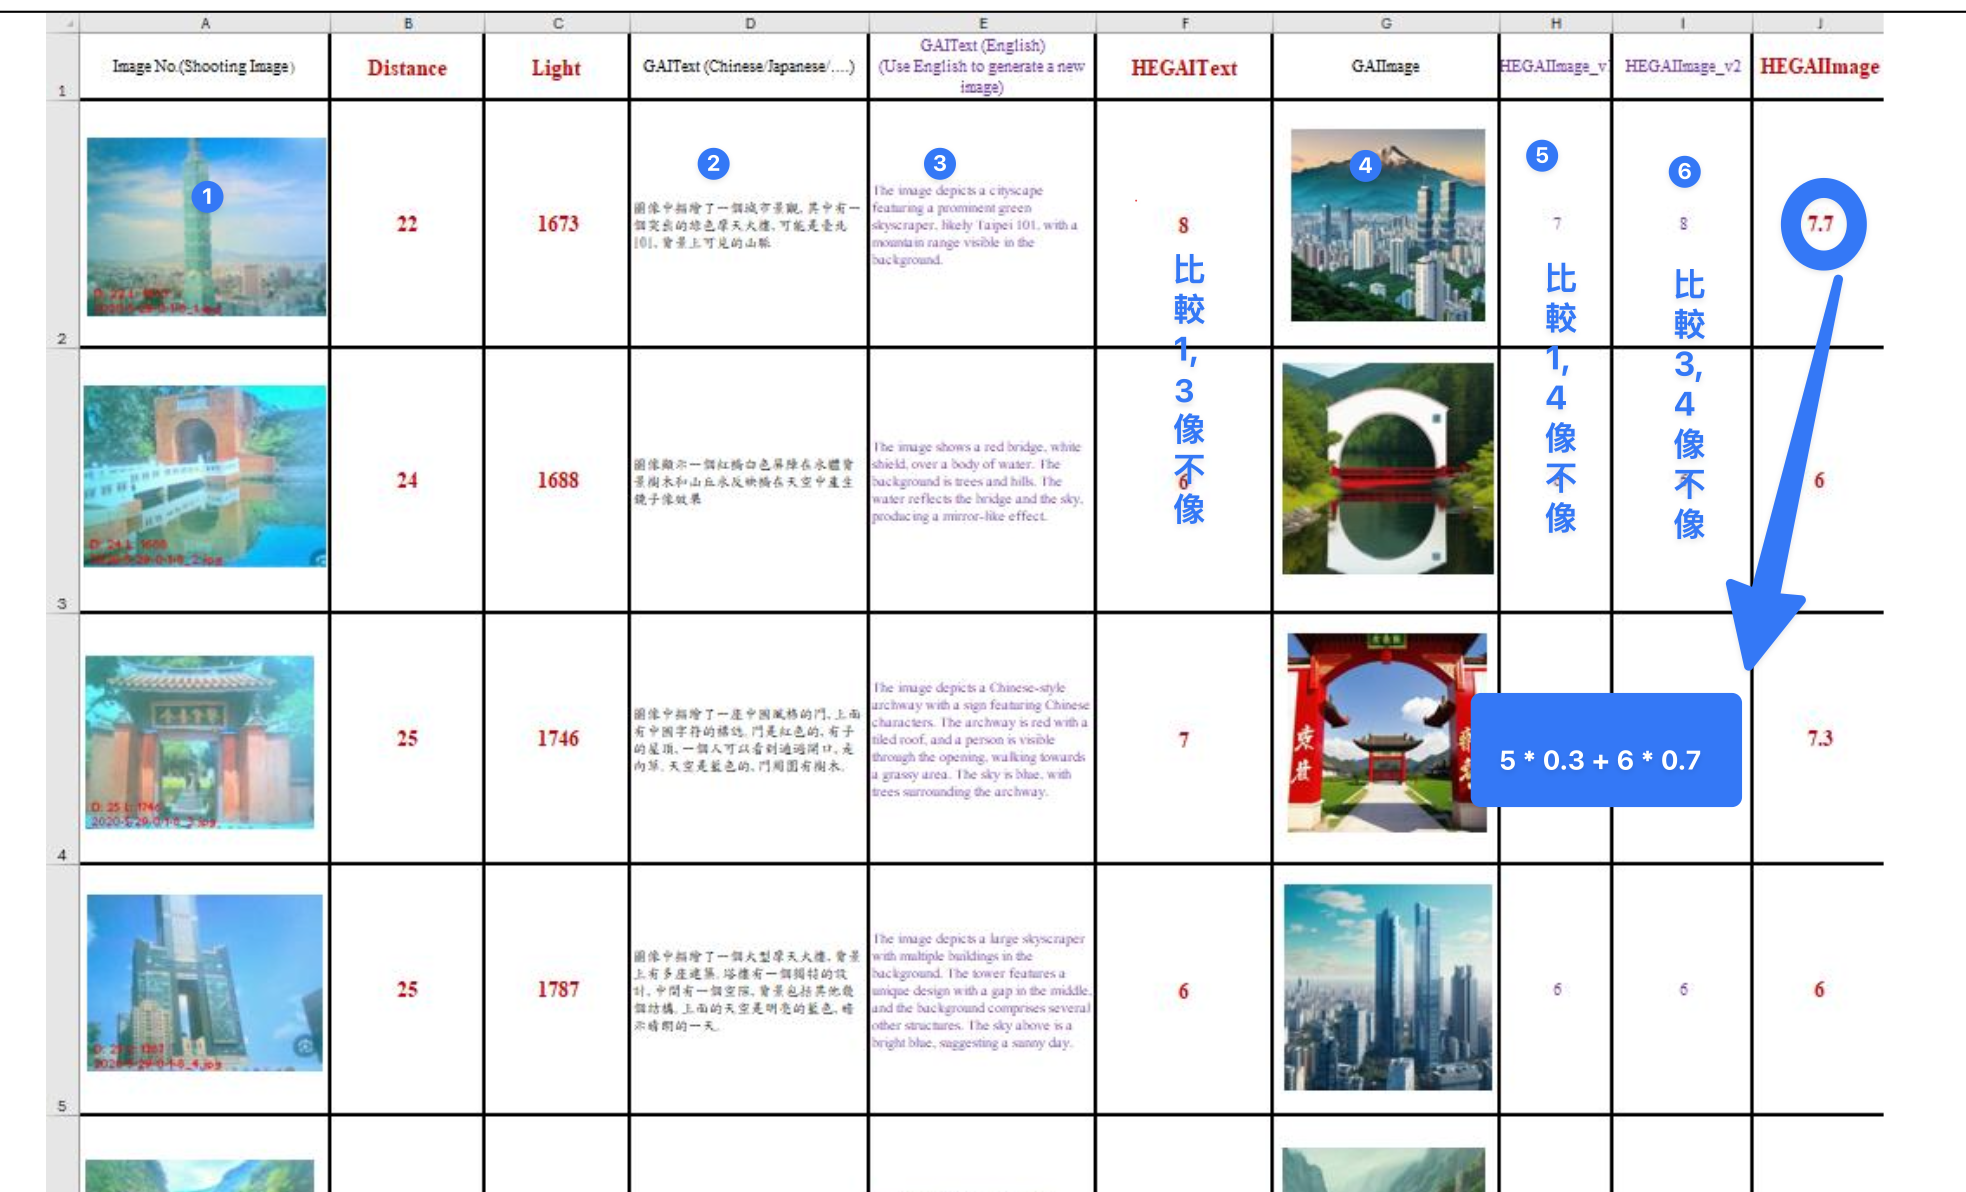
\includegraphics[width=0.45\textwidth]{res/image/labeling_train_data.png} % Replace image1.png with your image file
    \caption{學習資料標記} % Optional caption
    \label{fig:labeling_dataset} % Optional label
\end{figure}

\begin{figure}[htbp]
    \centering
    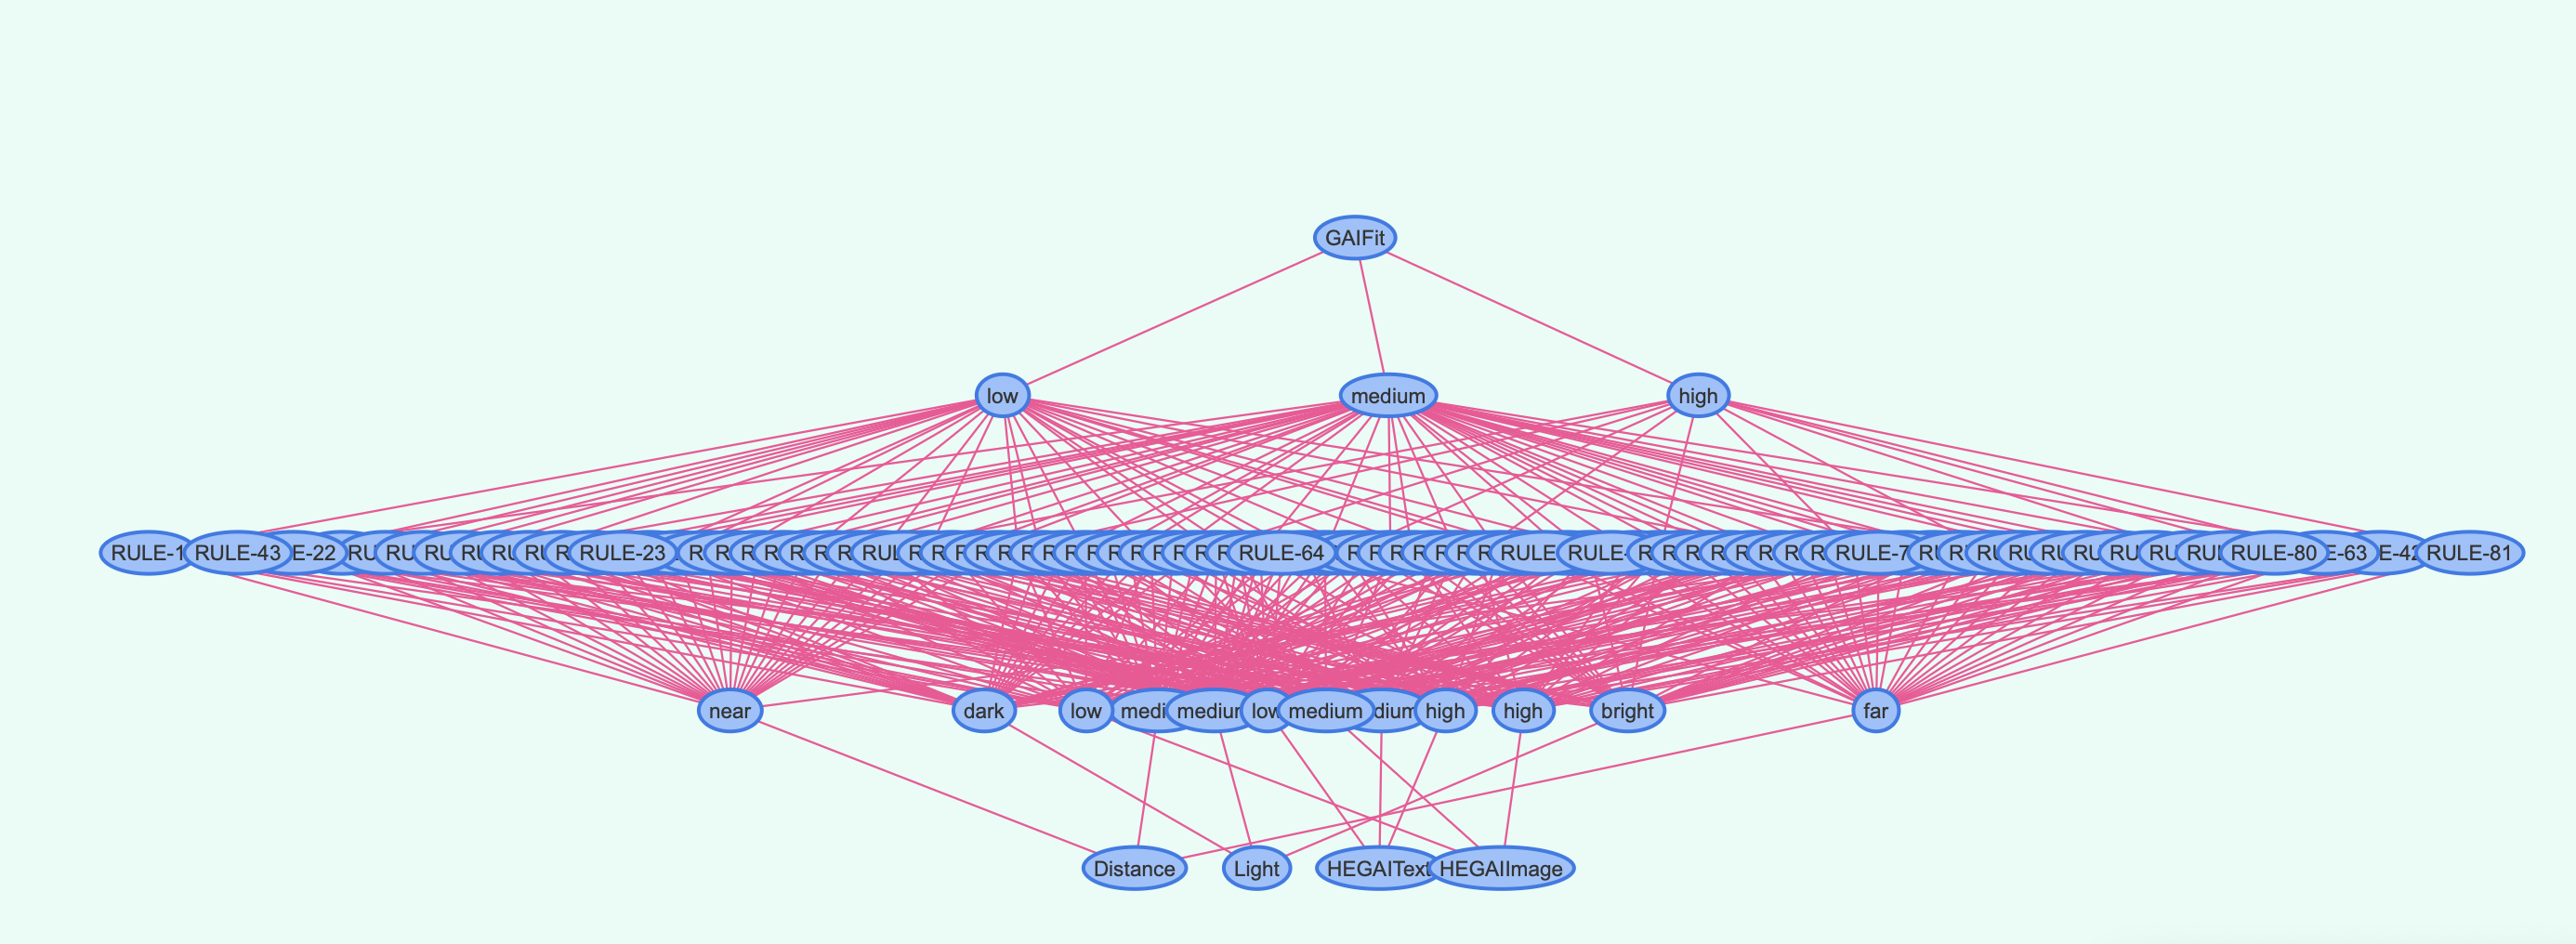
\includegraphics[width=0.45\textwidth]{res/image/model.png} % Replace image2.png with your image file
    \caption{模型} % Optional caption
    \label{fig:model}
\end{figure}

\begin{figure}[htbp]
    \centering
    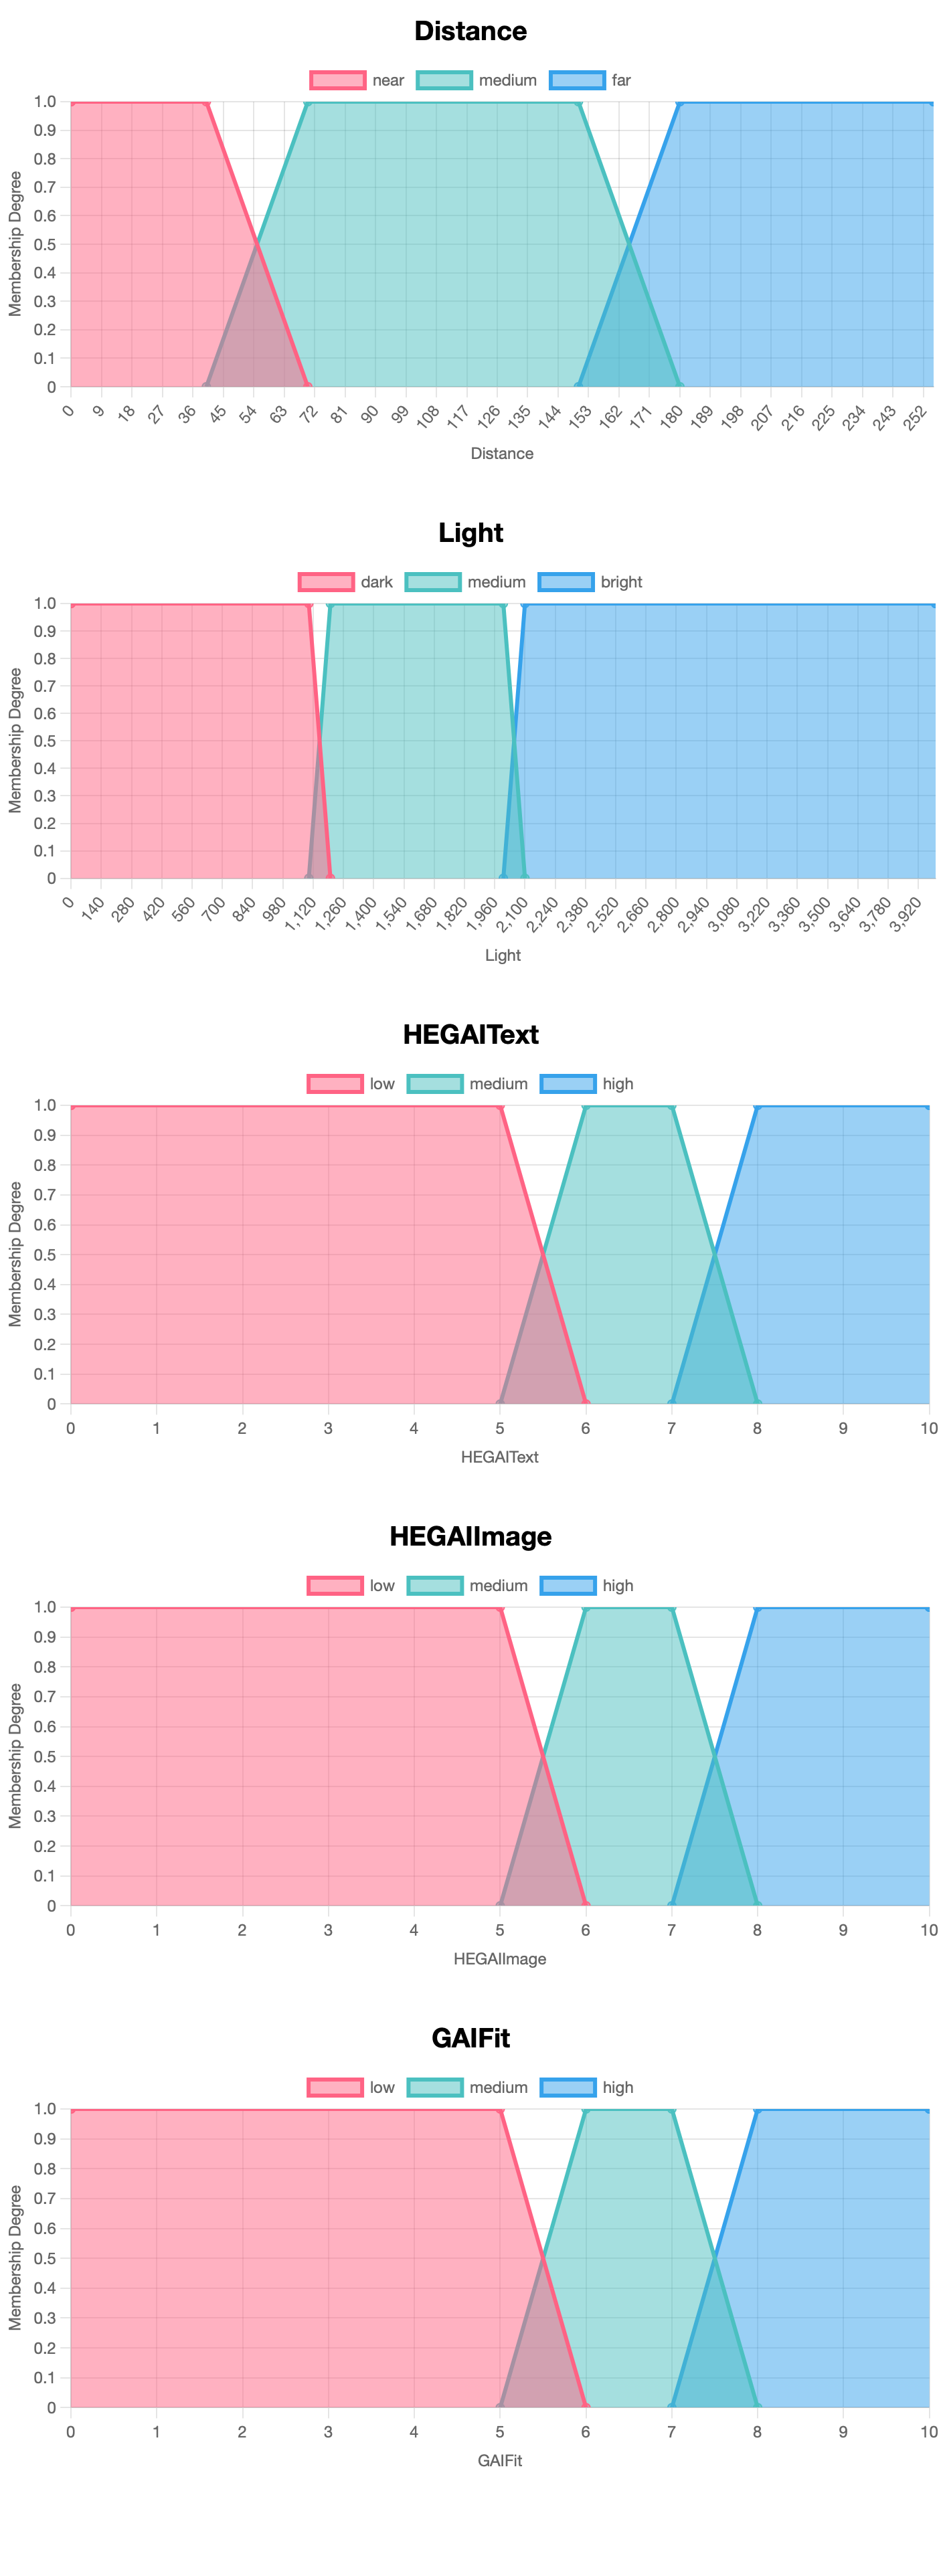
\includegraphics[width=0.45\textwidth]{res/image/all_BT.png} % Replace image3.png with your image file
    \caption{訓練前 T 型圖}
    \label{fig:all_BT}  
\end{figure}

\begin{figure}[htbp]
    \centering
    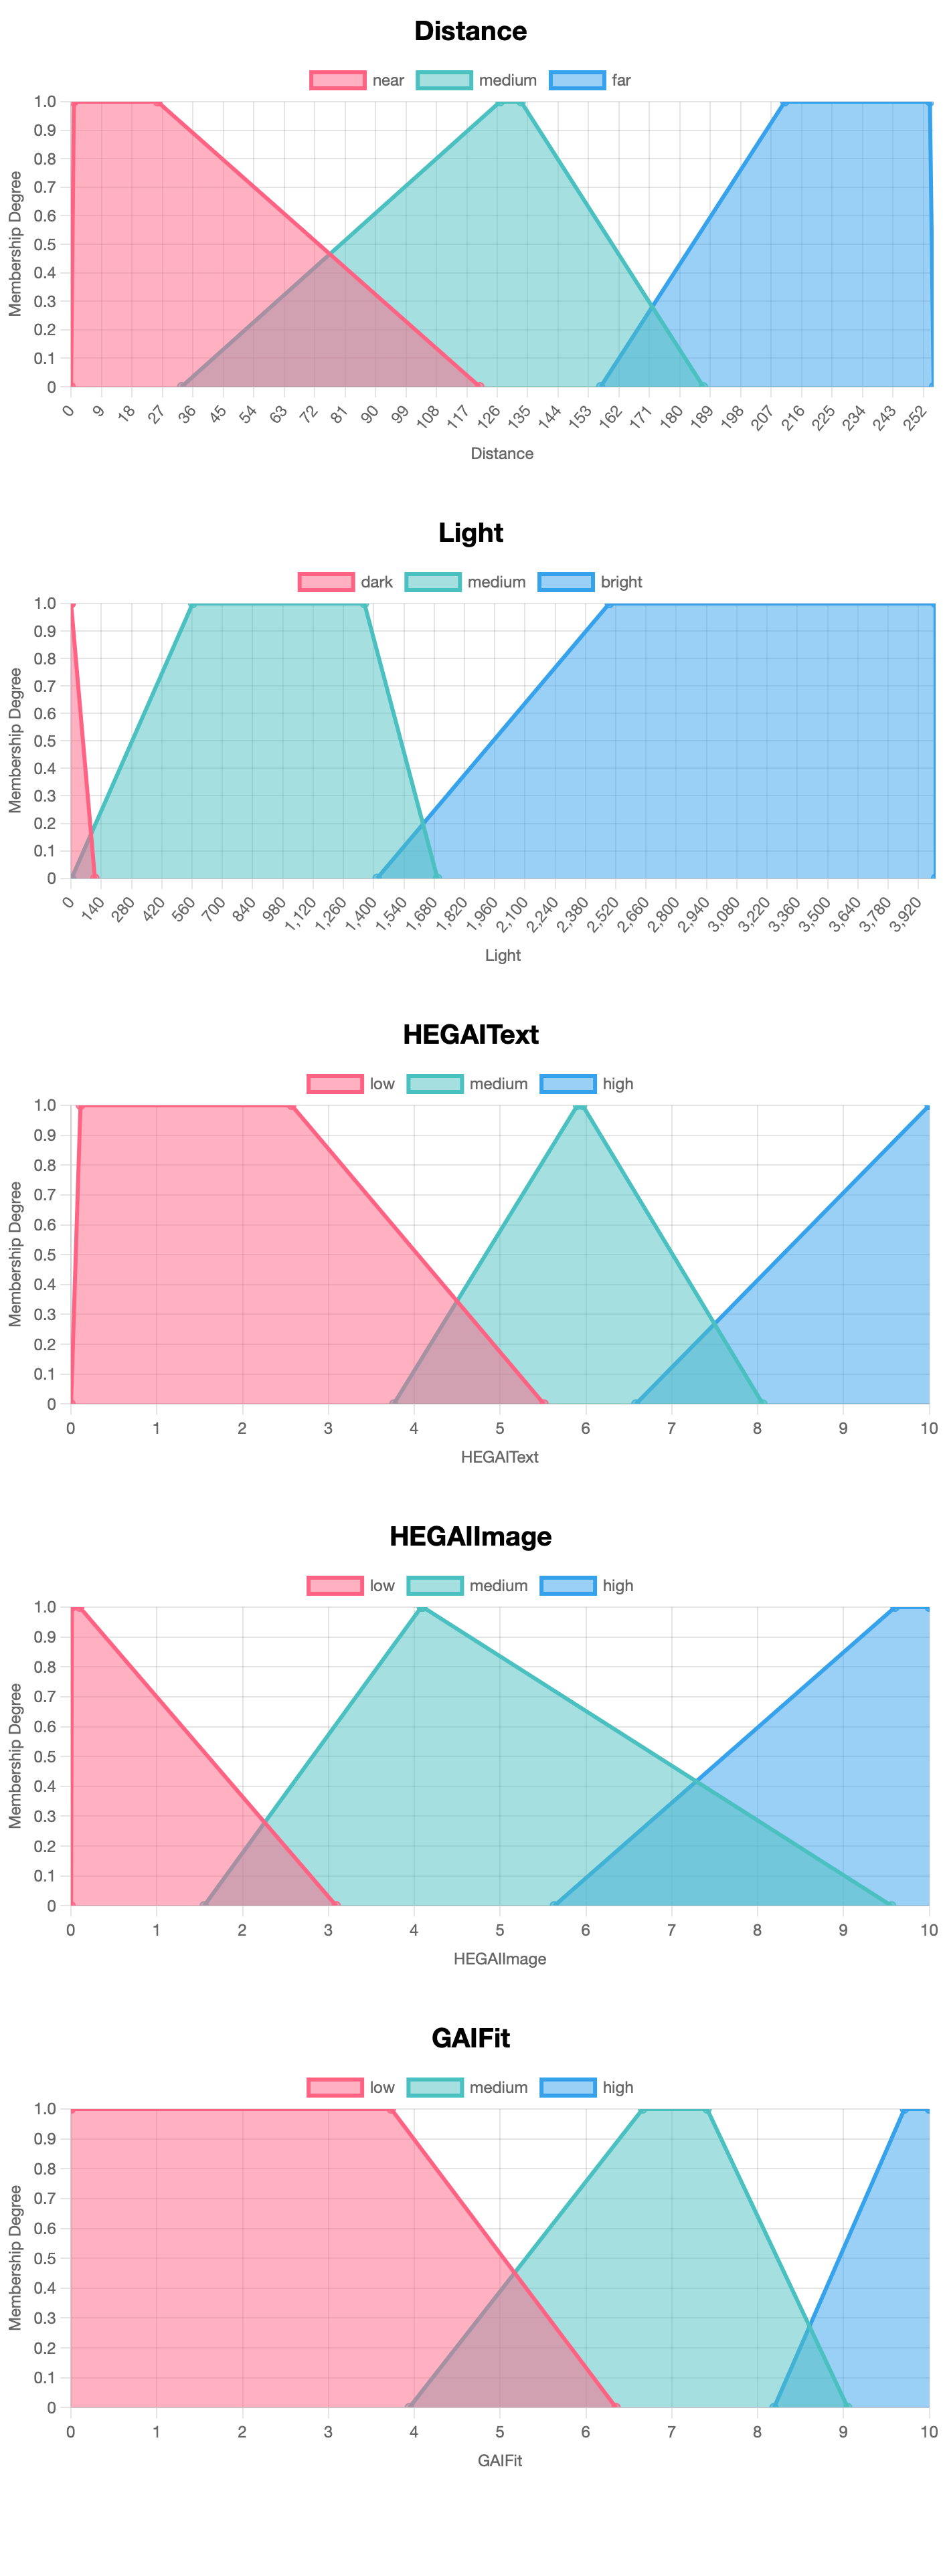
\includegraphics[width=0.45\textwidth]{res/image/all_AL.png} % Replace image3.png with your image file
    \caption{訓練會 T 型圖}
    \label{fig:all_AL}  
\end{figure}

\begin{figure}[htbp]
    \centering
    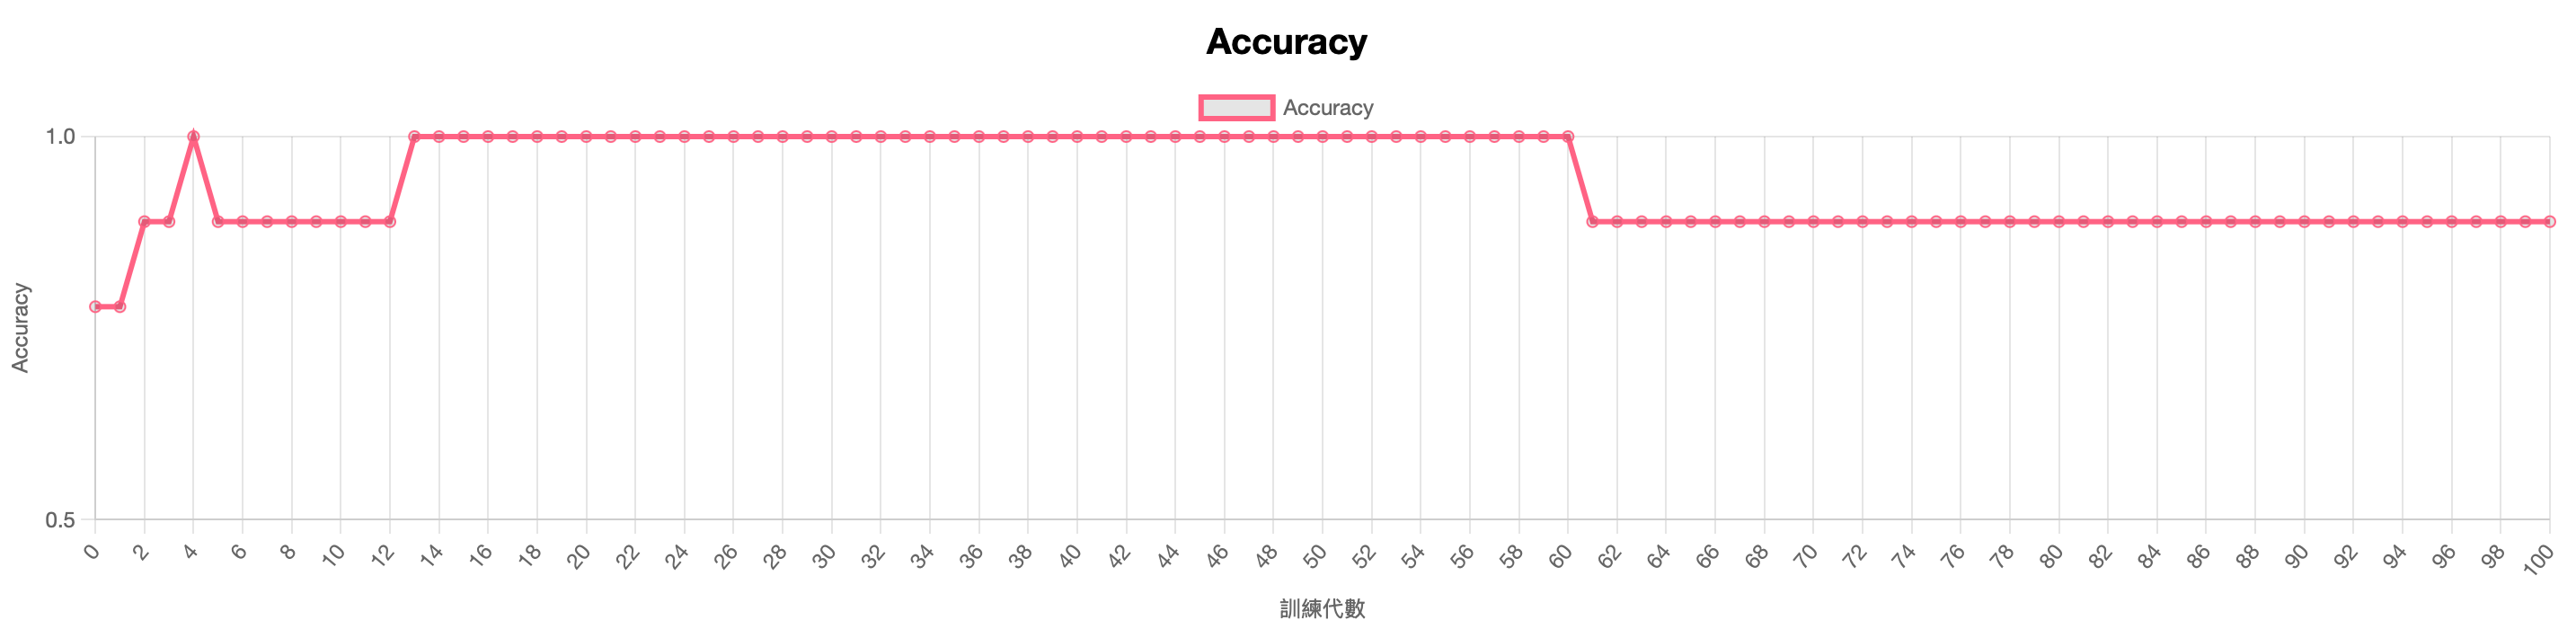
\includegraphics[width=0.45\textwidth]{res/image/accuracy.png} % Replace image4.png with your image file
    \caption{Accuracy Curve} % Optional caption
    \label{fig:accuracy_curve} % Optional label
\end{figure}

\begin{figure}[htbp]
    \centering
    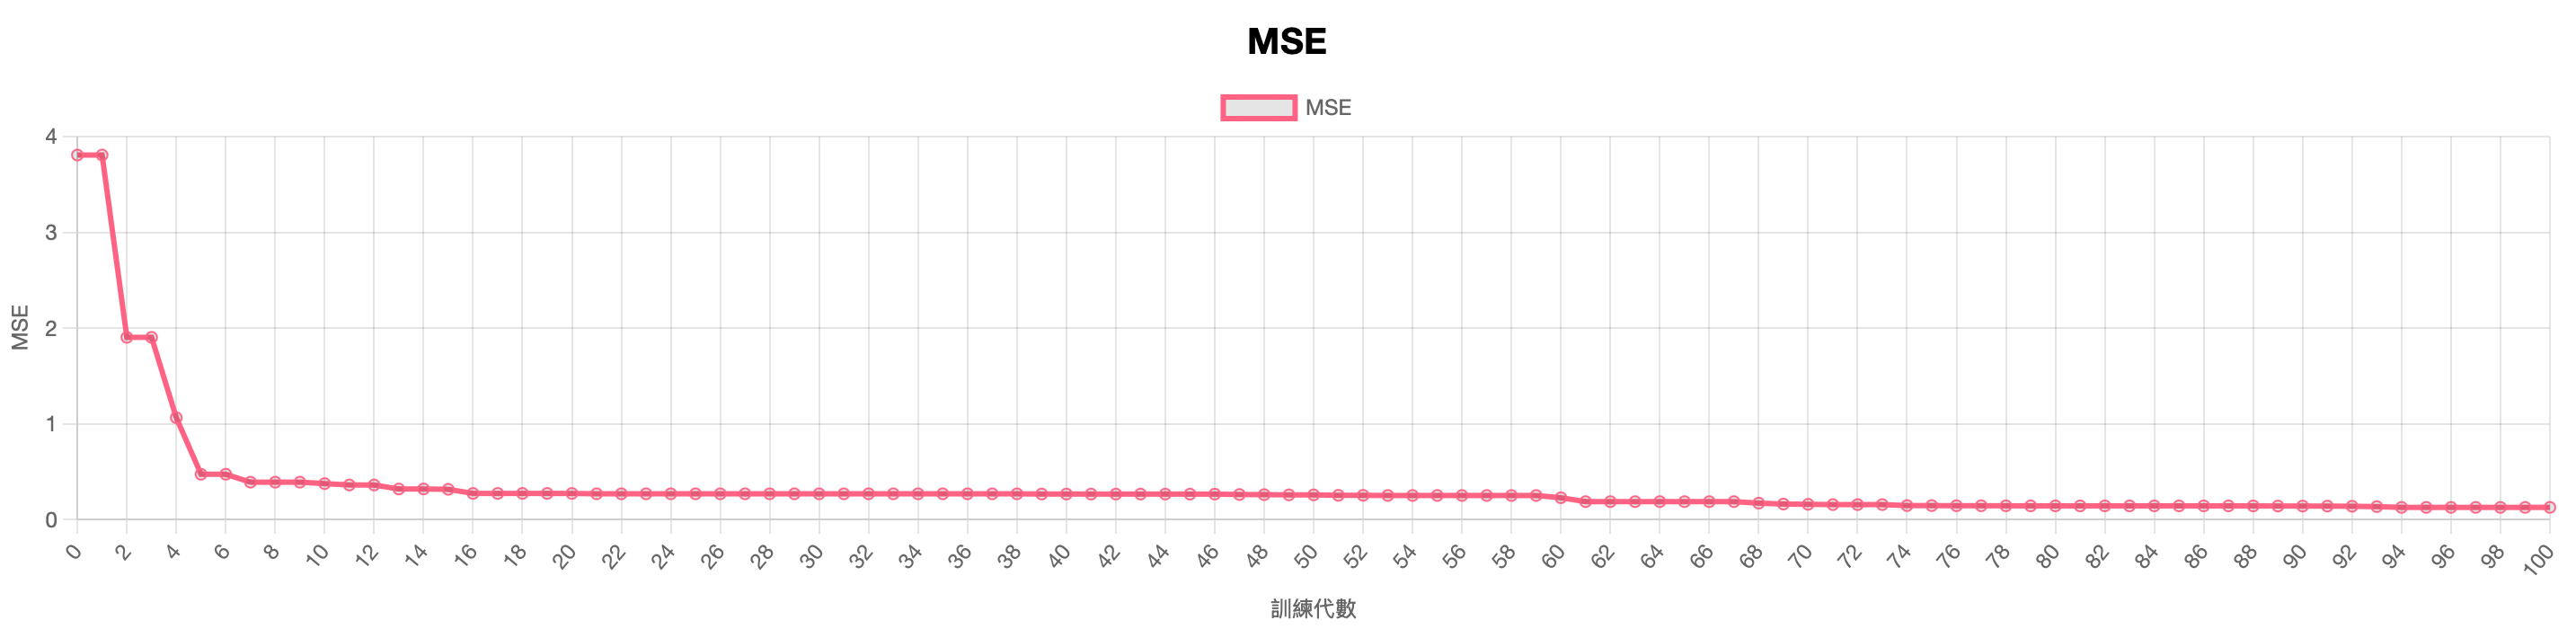
\includegraphics[width=0.45\textwidth]{res/image/mse.png} % Replace image5.png with your image file
    \caption{MSE Curve} % Optional caption
    \label{fig:mse_curve} % Optional label
\end{figure}

\begin{figure}[htbp]
    \centering
    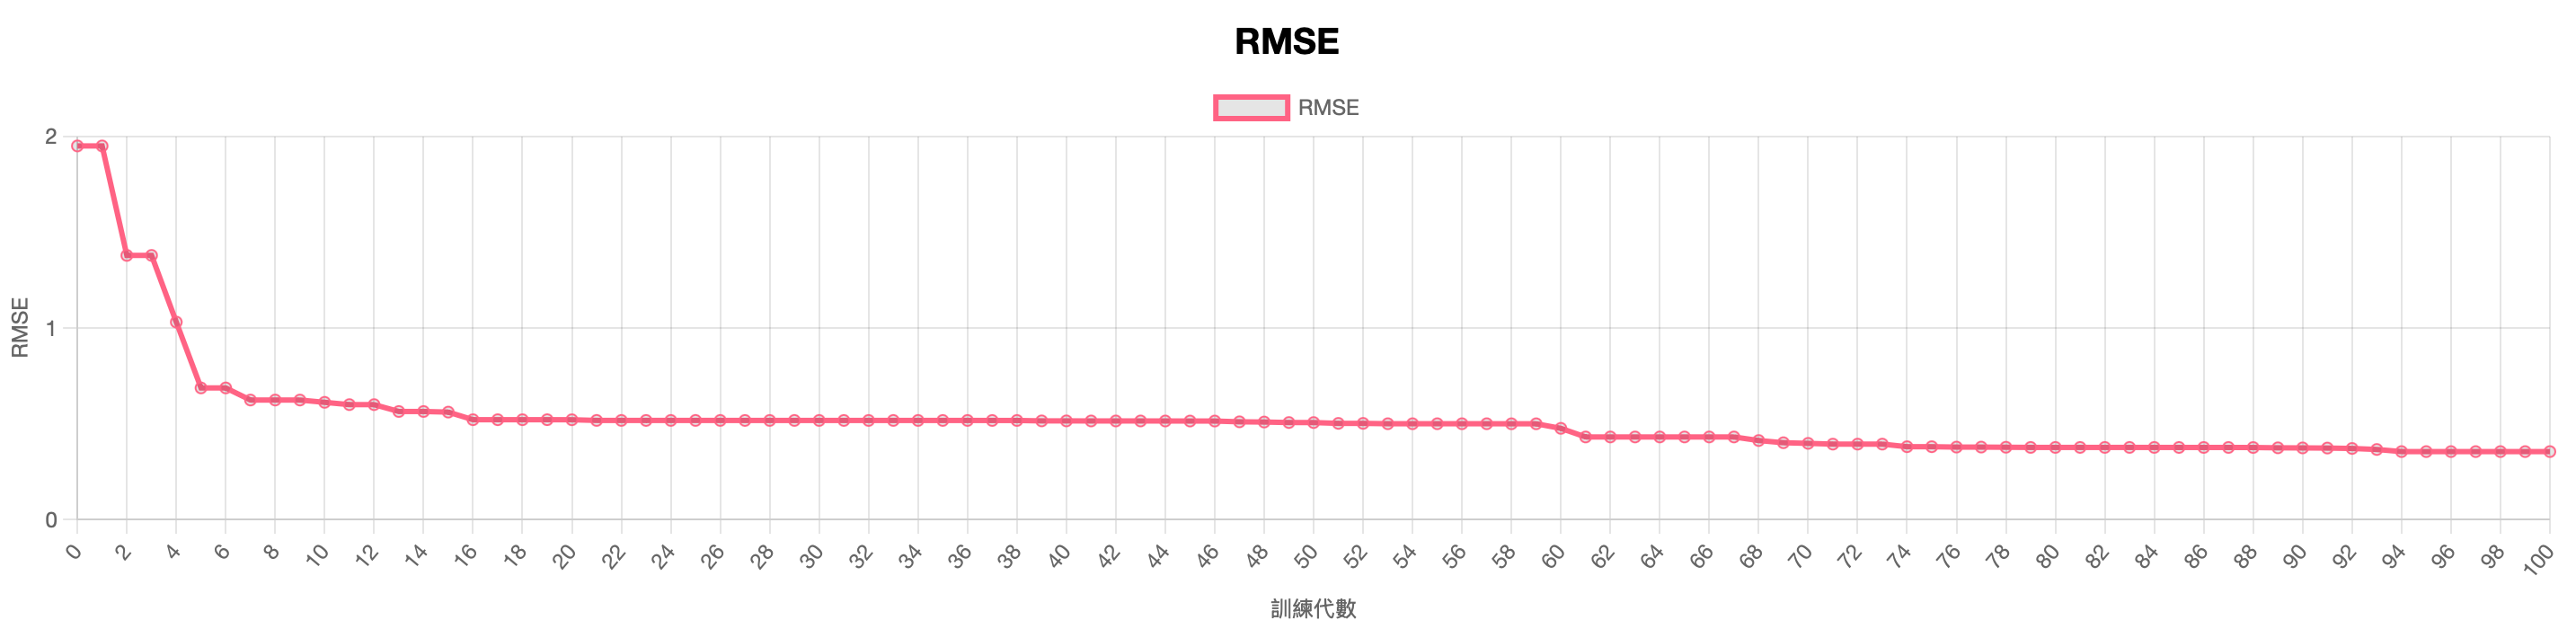
\includegraphics[width=0.45\textwidth]{res/image/rmse.png} % Replace image5.png with your image file
    \caption{RMSE Curve} % Optional caption
    \label{fig:rmse_curve} % Optional label
\end{figure}


\begin{figure}[htbp]
    \centering
    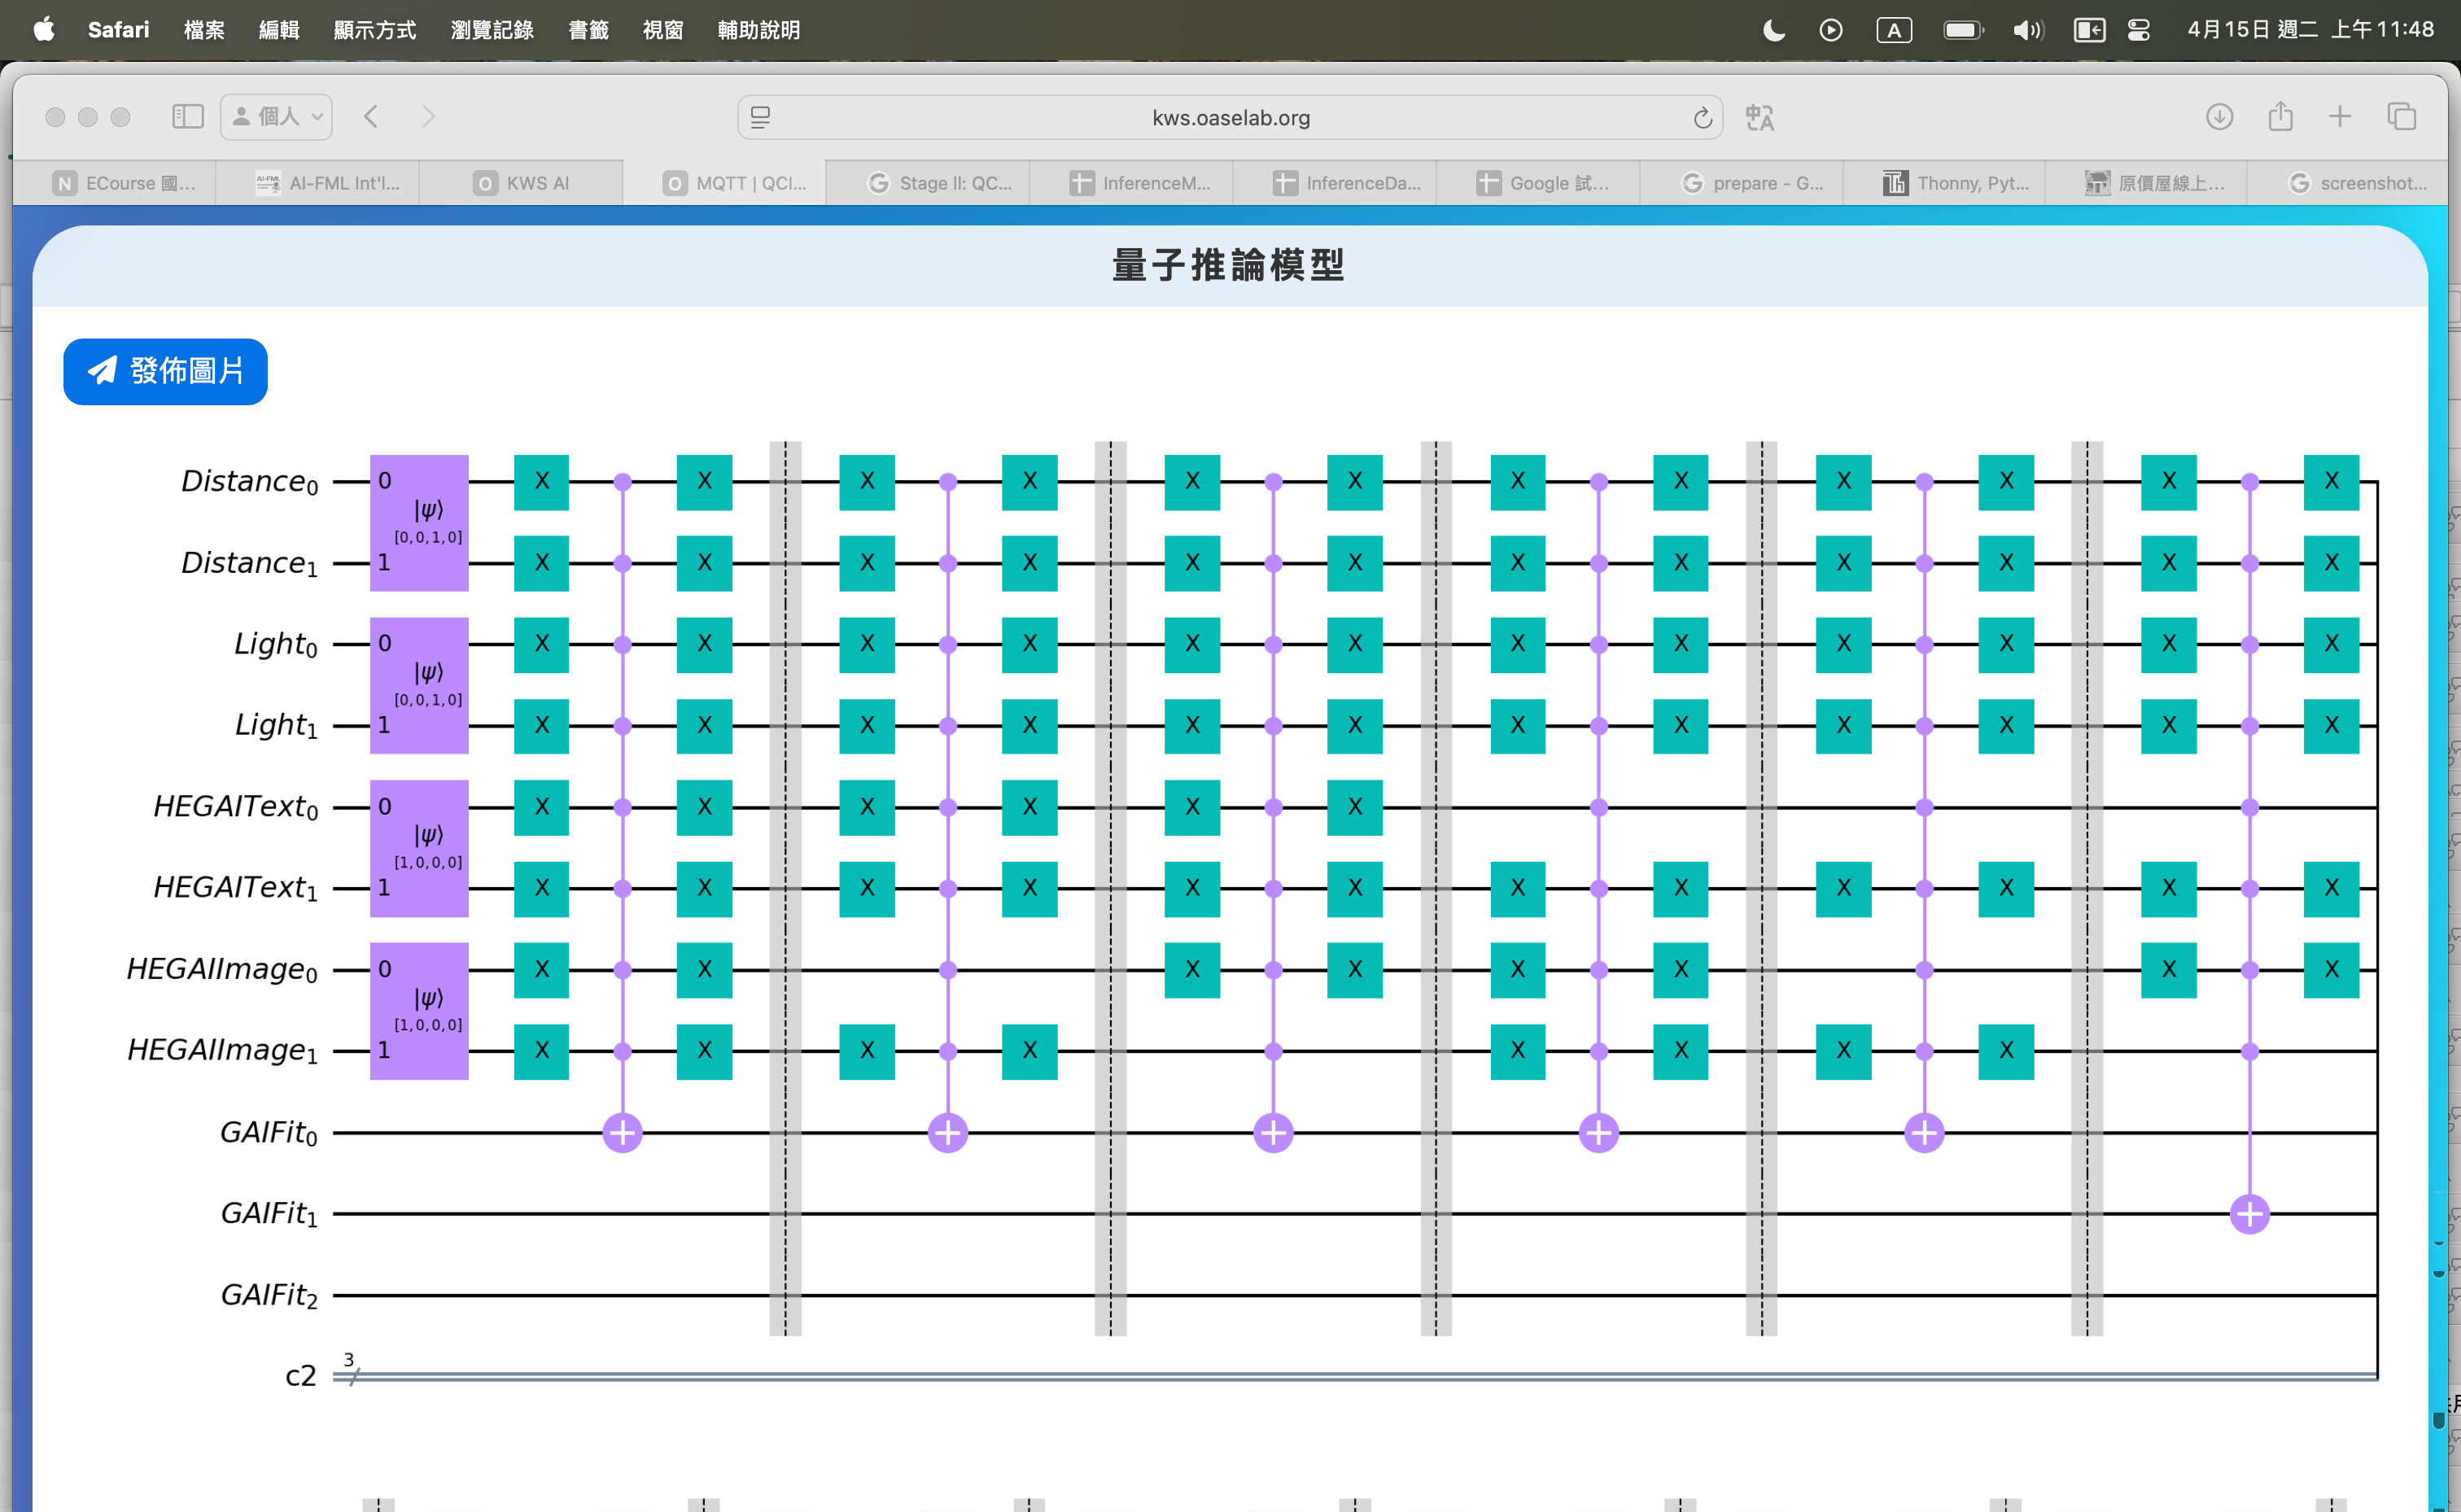
\includegraphics[width=0.45\textwidth]{res/image/quantum.png} % Replace image5.png with your image file
    \caption{量子電路實現} % Optional caption
    \label{fig:quantum_circuit} % Optional label
\end{figure}
\FloatBarrier %

\section{心得影片}
\href{https://youtu.be/spqwshHfivA}{https://youtu.be/spqwshHfivA}


% Section: Conclusion
\section{結論}
本報告成功地將軟體工程的核心理論與 QCI\&AI 學習工具的實際操作相結合,建立了一個綜合性的學習框架。透過回顧軟體工程導論、軟體流程、敏捷開發和需求工程等基本概念,並詳細闡述了 Kuwa 平台(涵蓋不同安裝環境)、Gemini Pro API 整合、本地 GGUF 模型部署(包括 Docker 化部署)以及 RAG 功能的配置與應用,我們展示了軟體工程原則如何在 QCI\&AI 的學習過程中提供指導。

將 IEEE SSCI 2025 工作坊倡導的數據收集、推論模型和微調模型學習階段與軟體工程的需求工程、設計實現、驗證和演進等活動相聯繫,可以幫助學習者更有條理地進行探索和實驗。例如,選擇雲端/本地模型或 RAG 類似於技術選型,評估模型輸出類似於軟體測試,而 Prompt Engineering、RAG 知識庫維護和對微調的理解則體現了敏捷迭代和軟體演進的思想。

總之,在學習和應用 QCI\&AI 這類快速發展的技術時,紮實的軟體工程基礎不僅不是束縛,反而是重要的助推器。它能幫助我們結構化問題、管理複雜性、評估方案、驗證結果,並以更系統化的方式應對技術挑戰,從而更有效地駕馭 AI 與量子計算融合帶來的機遇。


\section*{感謝名單}
在此,我衷心感謝以下人員對本報告的貢獻與支持:
\begin{itemize}[noitemsep, topsep=0pt]
    \item \textbf{李健興教授}:在軟體工程和 QCI\&AI 領域的專業指導和啟發。
    \item \textbf{KuwaAI 團隊}:提供 Kuwa 平台和相關技術支援,使本報告的實作部分得以順利進行。
    \item \textbf{TAIDE 團隊}:提供 TAIDE 模型和相關技術支援。
    \item \textbf{所有參與討論和提供建議的同學}:你們的意見和反饋對本報告的完善至關重要。
\end{itemize}


% References
\begin{thebibliography}{9}

\bibitem{sommerville2015}
Sommerville, I. (2015). \textit{Software Engineering} (10th ed.). Pearson.

\bibitem{kuwa_github}
KuwaAI. (n.d.). \textit{GenAI OS}. GitHub Repository. Retrieved from \url{https://github.com/kuwaai/genai-os}

\end{thebibliography}

\end{document}
